% Options for packages loaded elsewhere
\PassOptionsToPackage{unicode}{hyperref}
\PassOptionsToPackage{hyphens}{url}
%
\documentclass[
]{article}
\usepackage{amsmath,amssymb}
\usepackage{lmodern}
\usepackage{iftex}
\ifPDFTeX
  \usepackage[T1]{fontenc}
  \usepackage[utf8]{inputenc}
  \usepackage{textcomp} % provide euro and other symbols
\else % if luatex or xetex
  \usepackage{unicode-math}
  \defaultfontfeatures{Scale=MatchLowercase}
  \defaultfontfeatures[\rmfamily]{Ligatures=TeX,Scale=1}
\fi
% Use upquote if available, for straight quotes in verbatim environments
\IfFileExists{upquote.sty}{\usepackage{upquote}}{}
\IfFileExists{microtype.sty}{% use microtype if available
  \usepackage[]{microtype}
  \UseMicrotypeSet[protrusion]{basicmath} % disable protrusion for tt fonts
}{}
\makeatletter
\@ifundefined{KOMAClassName}{% if non-KOMA class
  \IfFileExists{parskip.sty}{%
    \usepackage{parskip}
  }{% else
    \setlength{\parindent}{0pt}
    \setlength{\parskip}{6pt plus 2pt minus 1pt}}
}{% if KOMA class
  \KOMAoptions{parskip=half}}
\makeatother
\usepackage{xcolor}
\usepackage[margin=1in]{geometry}
\usepackage{color}
\usepackage{fancyvrb}
\newcommand{\VerbBar}{|}
\newcommand{\VERB}{\Verb[commandchars=\\\{\}]}
\DefineVerbatimEnvironment{Highlighting}{Verbatim}{commandchars=\\\{\}}
% Add ',fontsize=\small' for more characters per line
\usepackage{framed}
\definecolor{shadecolor}{RGB}{248,248,248}
\newenvironment{Shaded}{\begin{snugshade}}{\end{snugshade}}
\newcommand{\AlertTok}[1]{\textcolor[rgb]{0.94,0.16,0.16}{#1}}
\newcommand{\AnnotationTok}[1]{\textcolor[rgb]{0.56,0.35,0.01}{\textbf{\textit{#1}}}}
\newcommand{\AttributeTok}[1]{\textcolor[rgb]{0.77,0.63,0.00}{#1}}
\newcommand{\BaseNTok}[1]{\textcolor[rgb]{0.00,0.00,0.81}{#1}}
\newcommand{\BuiltInTok}[1]{#1}
\newcommand{\CharTok}[1]{\textcolor[rgb]{0.31,0.60,0.02}{#1}}
\newcommand{\CommentTok}[1]{\textcolor[rgb]{0.56,0.35,0.01}{\textit{#1}}}
\newcommand{\CommentVarTok}[1]{\textcolor[rgb]{0.56,0.35,0.01}{\textbf{\textit{#1}}}}
\newcommand{\ConstantTok}[1]{\textcolor[rgb]{0.00,0.00,0.00}{#1}}
\newcommand{\ControlFlowTok}[1]{\textcolor[rgb]{0.13,0.29,0.53}{\textbf{#1}}}
\newcommand{\DataTypeTok}[1]{\textcolor[rgb]{0.13,0.29,0.53}{#1}}
\newcommand{\DecValTok}[1]{\textcolor[rgb]{0.00,0.00,0.81}{#1}}
\newcommand{\DocumentationTok}[1]{\textcolor[rgb]{0.56,0.35,0.01}{\textbf{\textit{#1}}}}
\newcommand{\ErrorTok}[1]{\textcolor[rgb]{0.64,0.00,0.00}{\textbf{#1}}}
\newcommand{\ExtensionTok}[1]{#1}
\newcommand{\FloatTok}[1]{\textcolor[rgb]{0.00,0.00,0.81}{#1}}
\newcommand{\FunctionTok}[1]{\textcolor[rgb]{0.00,0.00,0.00}{#1}}
\newcommand{\ImportTok}[1]{#1}
\newcommand{\InformationTok}[1]{\textcolor[rgb]{0.56,0.35,0.01}{\textbf{\textit{#1}}}}
\newcommand{\KeywordTok}[1]{\textcolor[rgb]{0.13,0.29,0.53}{\textbf{#1}}}
\newcommand{\NormalTok}[1]{#1}
\newcommand{\OperatorTok}[1]{\textcolor[rgb]{0.81,0.36,0.00}{\textbf{#1}}}
\newcommand{\OtherTok}[1]{\textcolor[rgb]{0.56,0.35,0.01}{#1}}
\newcommand{\PreprocessorTok}[1]{\textcolor[rgb]{0.56,0.35,0.01}{\textit{#1}}}
\newcommand{\RegionMarkerTok}[1]{#1}
\newcommand{\SpecialCharTok}[1]{\textcolor[rgb]{0.00,0.00,0.00}{#1}}
\newcommand{\SpecialStringTok}[1]{\textcolor[rgb]{0.31,0.60,0.02}{#1}}
\newcommand{\StringTok}[1]{\textcolor[rgb]{0.31,0.60,0.02}{#1}}
\newcommand{\VariableTok}[1]{\textcolor[rgb]{0.00,0.00,0.00}{#1}}
\newcommand{\VerbatimStringTok}[1]{\textcolor[rgb]{0.31,0.60,0.02}{#1}}
\newcommand{\WarningTok}[1]{\textcolor[rgb]{0.56,0.35,0.01}{\textbf{\textit{#1}}}}
\usepackage{graphicx}
\makeatletter
\def\maxwidth{\ifdim\Gin@nat@width>\linewidth\linewidth\else\Gin@nat@width\fi}
\def\maxheight{\ifdim\Gin@nat@height>\textheight\textheight\else\Gin@nat@height\fi}
\makeatother
% Scale images if necessary, so that they will not overflow the page
% margins by default, and it is still possible to overwrite the defaults
% using explicit options in \includegraphics[width, height, ...]{}
\setkeys{Gin}{width=\maxwidth,height=\maxheight,keepaspectratio}
% Set default figure placement to htbp
\makeatletter
\def\fps@figure{htbp}
\makeatother
\setlength{\emergencystretch}{3em} % prevent overfull lines
\providecommand{\tightlist}{%
  \setlength{\itemsep}{0pt}\setlength{\parskip}{0pt}}
\setcounter{secnumdepth}{-\maxdimen} % remove section numbering
\ifLuaTeX
  \usepackage{selnolig}  % disable illegal ligatures
\fi
\IfFileExists{bookmark.sty}{\usepackage{bookmark}}{\usepackage{hyperref}}
\IfFileExists{xurl.sty}{\usepackage{xurl}}{} % add URL line breaks if available
\urlstyle{same} % disable monospaced font for URLs
\hypersetup{
  pdftitle={Linear Models: Regression},
  pdfauthor={Isabelle Kirby, Bridgette Bryant},
  hidelinks,
  pdfcreator={LaTeX via pandoc}}

\title{Linear Models: Regression}
\author{Isabelle Kirby, Bridgette Bryant}
\date{}

\begin{document}
\maketitle

Linear Regression:

In simple terms, linear regression tries to predict a quantitative
target by fitting a linear model to the input of the predictors to best
fit the target in the training data. A simple linear regression model is
often in the form of y = wX + b where y values as the targets, X values
as the predictors, the linear model creates the weight matrix w and the
fitting parameter b. Linear models don't always have to be straight
lines, they can be complex polynomials with multiple predictor
variables. Once a linear regression model is created/trained, you can
judge it's performance by the standard error, t-value, and most of all
the p-value. A p-value very close to 0 is the most ideal, R will show
you with `***' to ' ' next to the value with `***' showing an excellent
p-value. Residual standard error is also another way to measure your
linear model, it calculated from residual sum of squared errors, and
measures the lack of fit the model has for the data. However, it is in
the units of the data and can be difficult to interpret at times,
therefore it is better to use r-squared which lies between 0 and 1. The
closer to 1 the better the model. You can also evaluate the model with
correlation, which shows the correlation, which shows the degree in
terms of 1 and -1, a close to 1 shows it is strongly positively
correlation, a -1 shows it is strongly negatively correlation, and
lastly a 0 shows no correlation. Linear regression has a few weaknesses
including iteration effects, where there is too much synergy between
predictors, causing them to have too much impact as a whole on the
model. Along with confounding variables, which correlate with both the
target and predictors which can give too high of a correlation in the
training data. Also, hidden variables in the model, this can lead to
false conclusions and assumptions such as a correlation being a
causation in the data. Linear regression is also very likely to underfit
data, causing it to fail at capturing some of the data and have a low
accuracy. However, linear regression is very simple to implement and has
a very high performance on linearly separable data sets. Also,
overfitting data is unlikely to happen and can be very easy to fix in
linear models using regularization.

We chose the ``Air\_Pollution.csv'' for this assignment. It contains
data of the overall air quality of different cities overtime.

It has 32191 observations initially.

\begin{Shaded}
\begin{Highlighting}[]
\NormalTok{df }\OtherTok{\textless{}{-}} \FunctionTok{read.csv}\NormalTok{(}\StringTok{"Air\_Pollution.csv"}\NormalTok{)}
\FunctionTok{str}\NormalTok{(df)}
\end{Highlighting}
\end{Shaded}

\begin{verbatim}
## 'data.frame':    32191 obs. of  10 variables:
##  $ Country.Name          : chr  "Afghanistan" "Albania" "Albania" "Albania" ...
##  $ City                  : chr  "Kabul" "Durres" "Durres" "Elbasan" ...
##  $ Year                  : int  2019 2015 2016 2015 2016 2017 2015 2016 2014 2015 ...
##  $ PM2.5                 : num  119.8 NA 14.3 NA NA ...
##  $ PM10                  : num  NA 17.6 24.6 NA NA ...
##  $ NO2                   : num  NA 26.6 24.8 24 26.3 ...
##  $ PM25.temporal.coverage: num  18 NA NA NA NA NA NA NA NA NA ...
##  $ PM10.temporal.coverage: num  NA NA NA NA NA NA NA NA NA NA ...
##  $ NO2.temporal.coverage : num  NA 84 87.9 97.9 96 ...
##  $ Updated.Year          : int  2022 2022 2022 2022 2022 2022 2022 2022 2022 2022 ...
\end{verbatim}

We then fill incomplete rows cells with the medians from their rows

\begin{Shaded}
\begin{Highlighting}[]
\NormalTok{df}\SpecialCharTok{$}\NormalTok{PM2}\FloatTok{.5}\NormalTok{[}\FunctionTok{is.na}\NormalTok{(df}\SpecialCharTok{$}\NormalTok{PM2}\FloatTok{.5}\NormalTok{)] }\OtherTok{\textless{}{-}} \FunctionTok{mean}\NormalTok{(df}\SpecialCharTok{$}\NormalTok{PM2}\FloatTok{.5}\NormalTok{, }\AttributeTok{na.rm=}\ConstantTok{TRUE}\NormalTok{)}
\NormalTok{df}\SpecialCharTok{$}\NormalTok{PM10[}\FunctionTok{is.na}\NormalTok{(df}\SpecialCharTok{$}\NormalTok{PM10)] }\OtherTok{\textless{}{-}} \FunctionTok{mean}\NormalTok{(df}\SpecialCharTok{$}\NormalTok{PM10, }\AttributeTok{na.rm=}\ConstantTok{TRUE}\NormalTok{)}
\NormalTok{df}\SpecialCharTok{$}\NormalTok{NO2[}\FunctionTok{is.na}\NormalTok{(df}\SpecialCharTok{$}\NormalTok{NO2)] }\OtherTok{\textless{}{-}} \FunctionTok{mean}\NormalTok{(df}\SpecialCharTok{$}\NormalTok{NO2, }\AttributeTok{na.rm=}\ConstantTok{TRUE}\NormalTok{)}
\NormalTok{df}\SpecialCharTok{$}\NormalTok{PM25.temporal.coverage[}\FunctionTok{is.na}\NormalTok{(df}\SpecialCharTok{$}\NormalTok{PM25.temporal.coverage)] }\OtherTok{\textless{}{-}}
  \FunctionTok{mean}\NormalTok{(df}\SpecialCharTok{$}\NormalTok{PM25.temporal.coverage, }\AttributeTok{na.rm=}\ConstantTok{TRUE}\NormalTok{)}
\NormalTok{df}\SpecialCharTok{$}\NormalTok{PM10.temporal.coverage[}\FunctionTok{is.na}\NormalTok{(df}\SpecialCharTok{$}\NormalTok{PM10.temporal.coverage)] }\OtherTok{\textless{}{-}}
  \FunctionTok{mean}\NormalTok{(df}\SpecialCharTok{$}\NormalTok{PM10.temporal.coverage, }\AttributeTok{na.rm=}\ConstantTok{TRUE}\NormalTok{)}
\NormalTok{df}\SpecialCharTok{$}\NormalTok{NO2.temporal.coverage[}\FunctionTok{is.na}\NormalTok{(df}\SpecialCharTok{$}\NormalTok{NO2.temporal.coverage)] }\OtherTok{\textless{}{-}}
  \FunctionTok{mean}\NormalTok{(df}\SpecialCharTok{$}\NormalTok{NO2.temporal.coverage, }\AttributeTok{na.rm=}\ConstantTok{TRUE}\NormalTok{)}

\FunctionTok{str}\NormalTok{(df)}
\end{Highlighting}
\end{Shaded}

\begin{verbatim}
## 'data.frame':    32191 obs. of  10 variables:
##  $ Country.Name          : chr  "Afghanistan" "Albania" "Albania" "Albania" ...
##  $ City                  : chr  "Kabul" "Durres" "Durres" "Elbasan" ...
##  $ Year                  : int  2019 2015 2016 2015 2016 2017 2015 2016 2014 2015 ...
##  $ PM2.5                 : num  119.8 22.9 14.3 22.9 22.9 ...
##  $ PM10                  : num  30.5 17.6 24.6 30.5 30.5 ...
##  $ NO2                   : num  20.6 26.6 24.8 24 26.3 ...
##  $ PM25.temporal.coverage: num  18 90.8 90.8 90.8 90.8 ...
##  $ PM10.temporal.coverage: num  90.6 90.6 90.6 90.6 90.6 ...
##  $ NO2.temporal.coverage : num  93.7 84 87.9 97.9 96 ...
##  $ Updated.Year          : int  2022 2022 2022 2022 2022 2022 2022 2022 2022 2022 ...
\end{verbatim}

Now we are creating the training and testing sets (80\% train, 20\%
test).

\begin{Shaded}
\begin{Highlighting}[]
\NormalTok{i }\OtherTok{\textless{}{-}}\FunctionTok{sample}\NormalTok{(}\DecValTok{1}\SpecialCharTok{:}\FunctionTok{nrow}\NormalTok{(df), }\FunctionTok{nrow}\NormalTok{(df)}\SpecialCharTok{*}\FloatTok{0.80}\NormalTok{, }\AttributeTok{replace=}\ConstantTok{FALSE}\NormalTok{)}
\NormalTok{train }\OtherTok{\textless{}{-}}\NormalTok{ df[i,]}
\NormalTok{test }\OtherTok{\textless{}{-}}\NormalTok{ df[}\SpecialCharTok{{-}}\NormalTok{i,]}
\end{Highlighting}
\end{Shaded}

\begin{Shaded}
\begin{Highlighting}[]
\FunctionTok{head}\NormalTok{(train)}
\end{Highlighting}
\end{Shaded}

\begin{verbatim}
##                   Country.Name            City Year    PM2.5     PM10      NO2
## 31858 United States of America Santa Rosa (Ca) 2016 22.92032 12.90000 20.61934
## 20686                   Mexico San Luis Potosi 2018 22.92032 30.53325 48.00000
## 28470              Switzerland        Montreux 2013 22.92032 30.53325 23.40000
## 13119                  Germany       Pirmasens 2010 22.92032 18.92000 24.85000
## 17478                    Italy           Cantu 2014 22.92032 27.43000 40.13000
## 19751                    Italy         Termoli 2018 22.92032 17.73000 18.53000
##       PM25.temporal.coverage PM10.temporal.coverage NO2.temporal.coverage
## 31858                90.7941                90.5835              93.69680
## 20686                90.7941                90.5835              88.76712
## 28470                90.7941                90.5835              93.69680
## 13119                90.7941                98.8810              93.90400
## 17478                90.7941                90.5835              96.03881
## 19751                90.7941                90.5835              95.15982
##       Updated.Year
## 31858         2022
## 20686         2022
## 28470         2022
## 13119         2022
## 17478         2022
## 19751         2022
\end{verbatim}

\begin{Shaded}
\begin{Highlighting}[]
\FunctionTok{tail}\NormalTok{(train)}
\end{Highlighting}
\end{Shaded}

\begin{verbatim}
##                   Country.Name                   City Year    PM2.5     PM10
## 19022                    Italy     Pignataro Maggiore 2017 22.92032 33.52000
## 26268                    Spain Los Corrales De Buelna 2013 22.92032 20.65000
## 17283                    Italy                 Bolano 2014 22.92032 30.53325
## 609                    Austria            Jennersdorf 2017 22.92032 20.62000
## 30439 United States of America Austin-Round Rock (Tx) 2018 22.92032 17.50000
## 23490                 Portugal                   Faro 2019 22.92032 17.49000
##         NO2 PM25.temporal.coverage PM10.temporal.coverage NO2.temporal.coverage
## 19022 32.64                90.7941                90.5835              94.98858
## 26268 15.93                90.7941                90.5835              99.28082
## 17283  6.07                90.7941                90.5835              86.30137
## 609   10.12                90.7941                90.5835              86.06164
## 30439  9.30                90.7941                90.5835              93.69680
## 23490  9.88                90.7941                90.5835              99.74886
##       Updated.Year
## 19022         2022
## 26268         2022
## 17283         2022
## 609           2022
## 30439         2022
## 23490         2022
\end{verbatim}

\begin{Shaded}
\begin{Highlighting}[]
\FunctionTok{range}\NormalTok{(train}\SpecialCharTok{$}\NormalTok{PM2}\FloatTok{.5}\NormalTok{, }\AttributeTok{na.rm=}\ConstantTok{FALSE}\NormalTok{)}
\end{Highlighting}
\end{Shaded}

\begin{verbatim}
## [1]   0.01 191.90
\end{verbatim}

\begin{Shaded}
\begin{Highlighting}[]
\FunctionTok{range}\NormalTok{(train}\SpecialCharTok{$}\NormalTok{PM10, }\AttributeTok{na.rm=}\ConstantTok{FALSE}\NormalTok{)}
\end{Highlighting}
\end{Shaded}

\begin{verbatim}
## [1]   1.04 540.00
\end{verbatim}

\begin{Shaded}
\begin{Highlighting}[]
\FunctionTok{mean}\NormalTok{(train}\SpecialCharTok{$}\NormalTok{PM2}\FloatTok{.5}\NormalTok{)}
\end{Highlighting}
\end{Shaded}

\begin{verbatim}
## [1] 22.91916
\end{verbatim}

\begin{Shaded}
\begin{Highlighting}[]
\FunctionTok{mean}\NormalTok{(train}\SpecialCharTok{$}\NormalTok{PM10)}
\end{Highlighting}
\end{Shaded}

\begin{verbatim}
## [1] 30.44424
\end{verbatim}

\begin{Shaded}
\begin{Highlighting}[]
\FunctionTok{median}\NormalTok{(train}\SpecialCharTok{$}\NormalTok{PM2}\FloatTok{.5}\NormalTok{)}
\end{Highlighting}
\end{Shaded}

\begin{verbatim}
## [1] 22.92032
\end{verbatim}

\begin{Shaded}
\begin{Highlighting}[]
\FunctionTok{median}\NormalTok{(train}\SpecialCharTok{$}\NormalTok{PM10)}
\end{Highlighting}
\end{Shaded}

\begin{verbatim}
## [1] 30.53325
\end{verbatim}

These are our plots

\begin{Shaded}
\begin{Highlighting}[]
\FunctionTok{hist}\NormalTok{(train}\SpecialCharTok{$}\NormalTok{PM2}\FloatTok{.5}\NormalTok{)}
\end{Highlighting}
\end{Shaded}

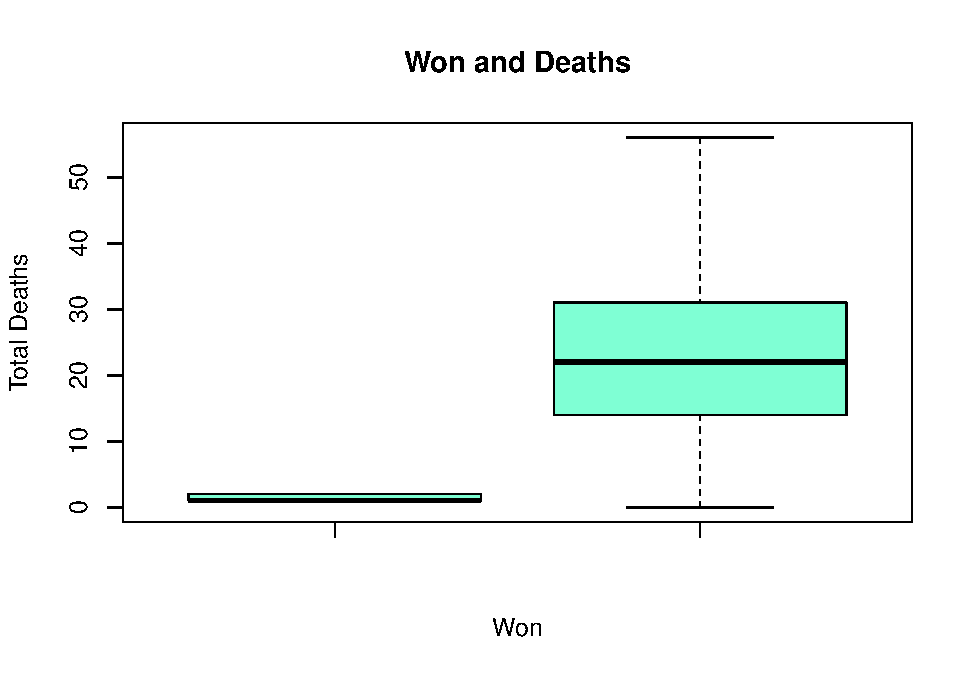
\includegraphics{Regression_files/figure-latex/unnamed-chunk-5-1.pdf}

\begin{Shaded}
\begin{Highlighting}[]
\FunctionTok{plot}\NormalTok{(train}\SpecialCharTok{$}\NormalTok{NO2, train}\SpecialCharTok{$}\NormalTok{Year)}
\end{Highlighting}
\end{Shaded}

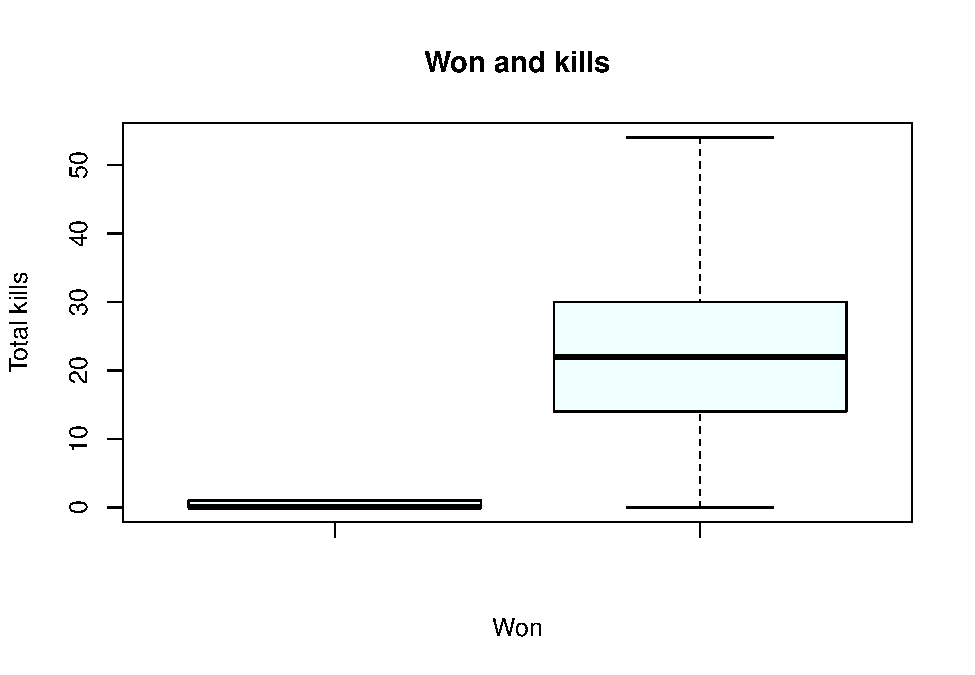
\includegraphics{Regression_files/figure-latex/unnamed-chunk-5-2.pdf}

\begin{Shaded}
\begin{Highlighting}[]
\FunctionTok{plot}\NormalTok{(train}\SpecialCharTok{$}\NormalTok{NO2, train}\SpecialCharTok{$}\NormalTok{PM2}\FloatTok{.5}\NormalTok{)}
\end{Highlighting}
\end{Shaded}

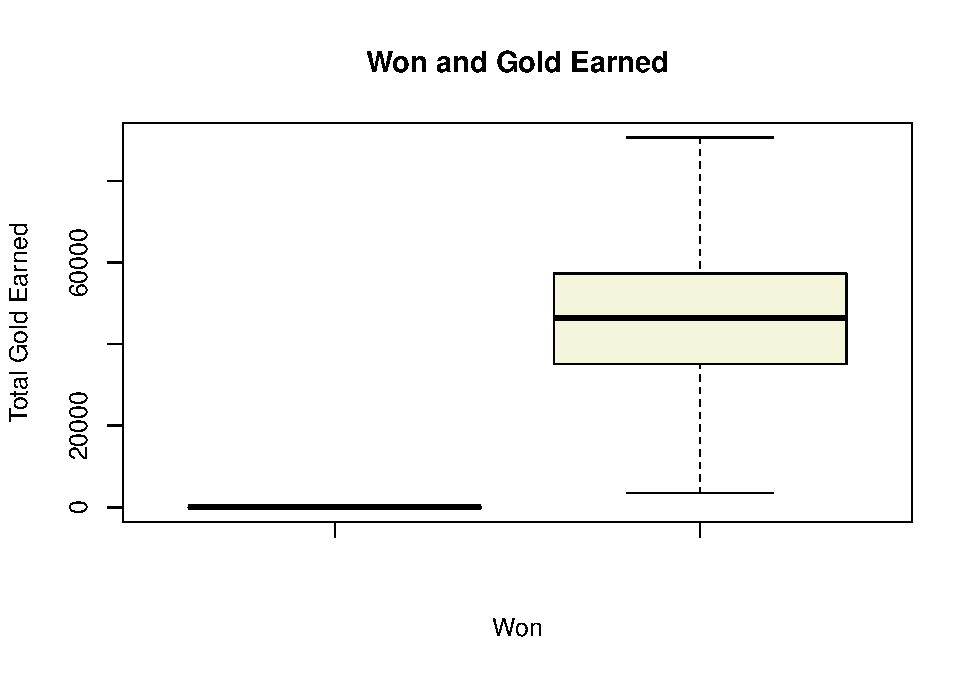
\includegraphics{Regression_files/figure-latex/unnamed-chunk-5-3.pdf}

\begin{Shaded}
\begin{Highlighting}[]
\FunctionTok{plot}\NormalTok{(train}\SpecialCharTok{$}\NormalTok{NO2, train}\SpecialCharTok{$}\NormalTok{PM10)}
\end{Highlighting}
\end{Shaded}

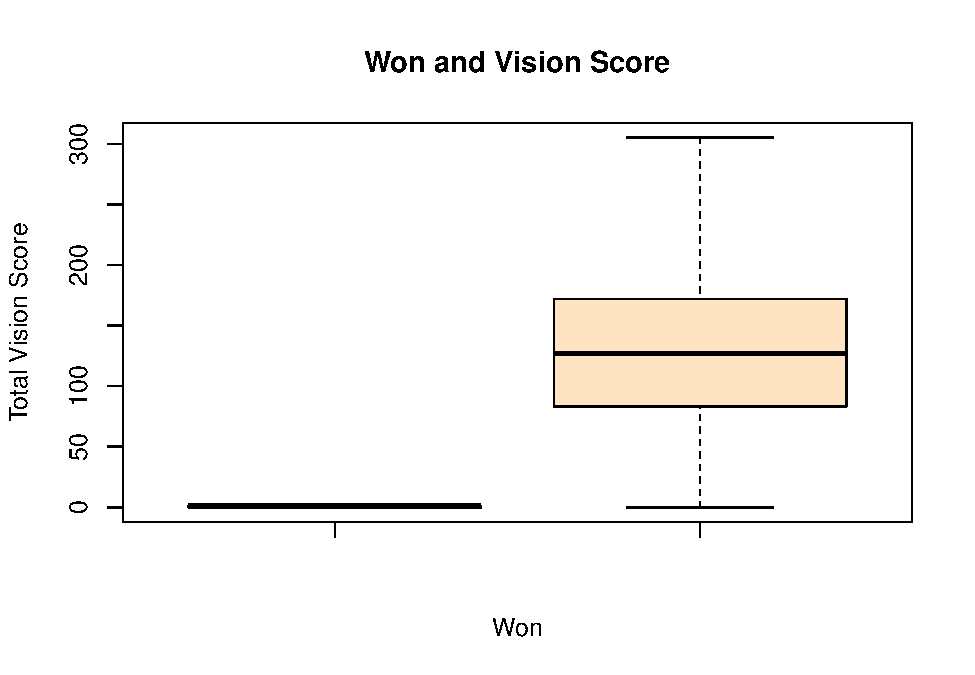
\includegraphics{Regression_files/figure-latex/unnamed-chunk-5-4.pdf}

Plotting the linear regression

\begin{Shaded}
\begin{Highlighting}[]
\NormalTok{lm1 }\OtherTok{\textless{}{-}} \FunctionTok{lm}\NormalTok{(NO2}\SpecialCharTok{\textasciitilde{}}\NormalTok{PM2}\FloatTok{.5}\NormalTok{, }\AttributeTok{data=}\NormalTok{train)}
\FunctionTok{summary}\NormalTok{(lm1)}
\end{Highlighting}
\end{Shaded}

\begin{verbatim}
## 
## Call:
## lm(formula = NO2 ~ PM2.5, data = train)
## 
## Residuals:
##     Min      1Q  Median      3Q     Max 
## -22.227  -5.556  -0.016   2.752 190.074 
## 
## Coefficients:
##              Estimate Std. Error t value Pr(>|t|)    
## (Intercept) 17.918618   0.131637  136.12   <2e-16 ***
## PM2.5        0.117231   0.005066   23.14   <2e-16 ***
## ---
## Signif. codes:  0 '***' 0.001 '**' 0.01 '*' 0.05 '.' 0.1 ' ' 1
## 
## Residual standard error: 9.95 on 25750 degrees of freedom
## Multiple R-squared:  0.02037,    Adjusted R-squared:  0.02033 
## F-statistic: 535.4 on 1 and 25750 DF,  p-value: < 2.2e-16
\end{verbatim}

The summary above is used to help determine if our linear model is good
or bad, if it accurately predicts our target or not. We can start with
the min, max, and median. As you can see it has a very wide range,
showing that we may have some outliers or very divided data. The
residual standard error is 9.974 on 25650 degrees of freedom, this
states that roughly the model's predictions are about 10 units off. The
multiple r-squared error is 0.02057, this should be as close to 1 as
possible. In most cases anything under .4 is a poor model at explaining
variance in the data. However our p-value is fairly low and very close
to 0, according to this we have a good model that is significant.

\begin{Shaded}
\begin{Highlighting}[]
\FunctionTok{plot}\NormalTok{(lm1)}
\end{Highlighting}
\end{Shaded}

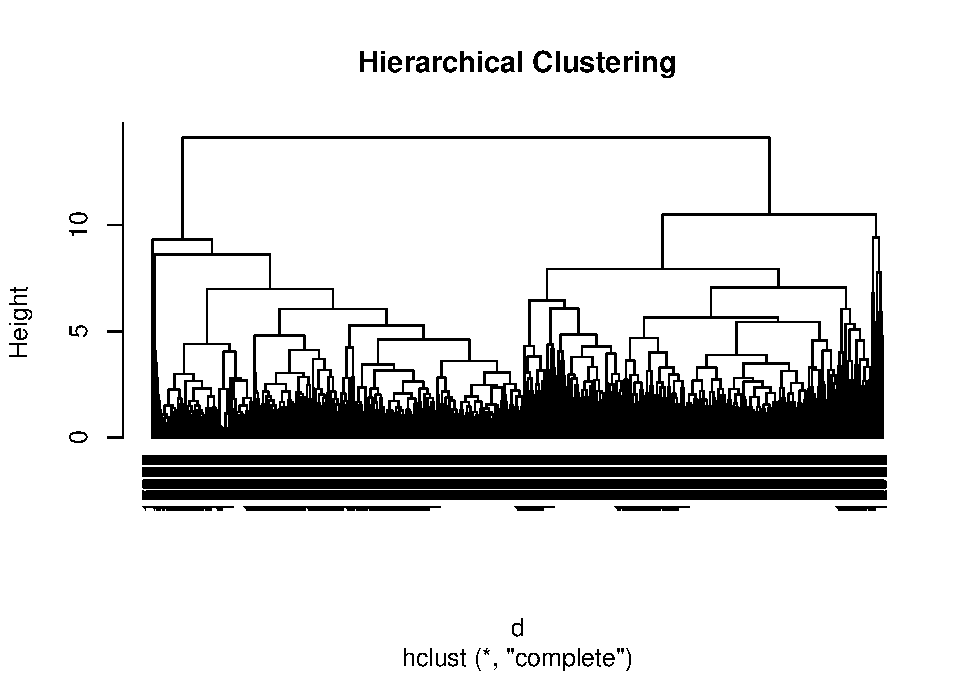
\includegraphics{Regression_files/figure-latex/unnamed-chunk-7-1.pdf}
\includegraphics{Regression_files/figure-latex/unnamed-chunk-7-2.pdf}
\includegraphics{Regression_files/figure-latex/unnamed-chunk-7-3.pdf}
\includegraphics{Regression_files/figure-latex/unnamed-chunk-7-4.pdf}

The residual plots above are summarized below:

Residuals vs Fitted: In this plot it shows whether the linearity holds,
indicated by the mean residual value for every fitted value region being
close to 0 (the red line being close to the dashed line). As you can see
the redline is very close to the dashed line close to 20, but drifts
downwards as we get close to 40 and 0. We can also see that we may have
outliers at point 16687 and the other two below (we cannot read them
because of the way R printed them ontop of eachother). Overall it shows
that our model is a good model.

Normal Q-Q: This graph shows the standardized residuals and theoretical
quantiles, if they come from the same distribution then the points
should form a roughly straight line. Our data set has a very straight
line until around (4, 10) where we once again see our outlier points
16687 and the couple below. As you can see it once again steers away
from the gray line in a strong curve shape. Although the line is still
fairly straight overall but we may have some skewed data in our dataset
(possibly from having to replace many missing values with the mean). It
can also mean since it is curved at the edge that our dataset contains
more extreme values.

Scale Location: Our scale-location graph is very uneven and is basically
a black blob. The residuals are supposed to be spread evenly across the
range of predictors, which can show the assumption of equal variance. As
you can tell ours is definitely not good, this shows that our assumption
of equal variance is very incorrect.

Leverage vs Residuals: In this plot the leverage is the extent to which
the coefficients in the regression model would change if a particular
observation was removed from the dataset. Thus observations with high
leverage have strong influence on the coefficients of the regression
model. The standardized residuals refer to the standardized difference
between a predicted value and actual value of an observation. You can
tell in the plots above that we have no influential points as all the
points of the data are within the cook's distance (dotted lines). But we
may have outliers at points 16563, 14785, and 1285.

\begin{Shaded}
\begin{Highlighting}[]
\NormalTok{lm2 }\OtherTok{\textless{}{-}} \FunctionTok{lm}\NormalTok{(NO2}\SpecialCharTok{\textasciitilde{}}\NormalTok{PM2}\FloatTok{.5}\SpecialCharTok{+}\NormalTok{PM10, }\AttributeTok{data=}\NormalTok{train)}
\FunctionTok{summary}\NormalTok{(lm2)}
\end{Highlighting}
\end{Shaded}

\begin{verbatim}
## 
## Call:
## lm(formula = NO2 ~ PM2.5 + PM10, data = train)
## 
## Residuals:
##     Min      1Q  Median      3Q     Max 
## -45.150  -5.462  -0.572   2.803 190.829 
## 
## Coefficients:
##              Estimate Std. Error t value Pr(>|t|)    
## (Intercept) 16.617712   0.138656  119.85   <2e-16 ***
## PM2.5        0.077283   0.005216   14.82   <2e-16 ***
## PM10         0.072805   0.002722   26.75   <2e-16 ***
## ---
## Signif. codes:  0 '***' 0.001 '**' 0.01 '*' 0.05 '.' 0.1 ' ' 1
## 
## Residual standard error: 9.815 on 25749 degrees of freedom
## Multiple R-squared:  0.04686,    Adjusted R-squared:  0.04678 
## F-statistic: 632.9 on 2 and 25749 DF,  p-value: < 2.2e-16
\end{verbatim}

The summary above can be used to compare this model with the previous
one above. The residual standard error is 9.82 instead of 9.974 on about
the same degrees of freedom, this states that roughly the model's
predictions are still about 10 units off but slightly less than the
previous model. The multiple r-squared error is 0.05059 instead of
0.02057, this should be as close to 1 as possible so it is very much an
improvement compared to the model above. However, it is still well under
.4 and therefore is still a poor model at explaining variance in the
data. The p-value is for both models is the same that is significant.

\begin{Shaded}
\begin{Highlighting}[]
\FunctionTok{plot}\NormalTok{(lm2)}
\end{Highlighting}
\end{Shaded}

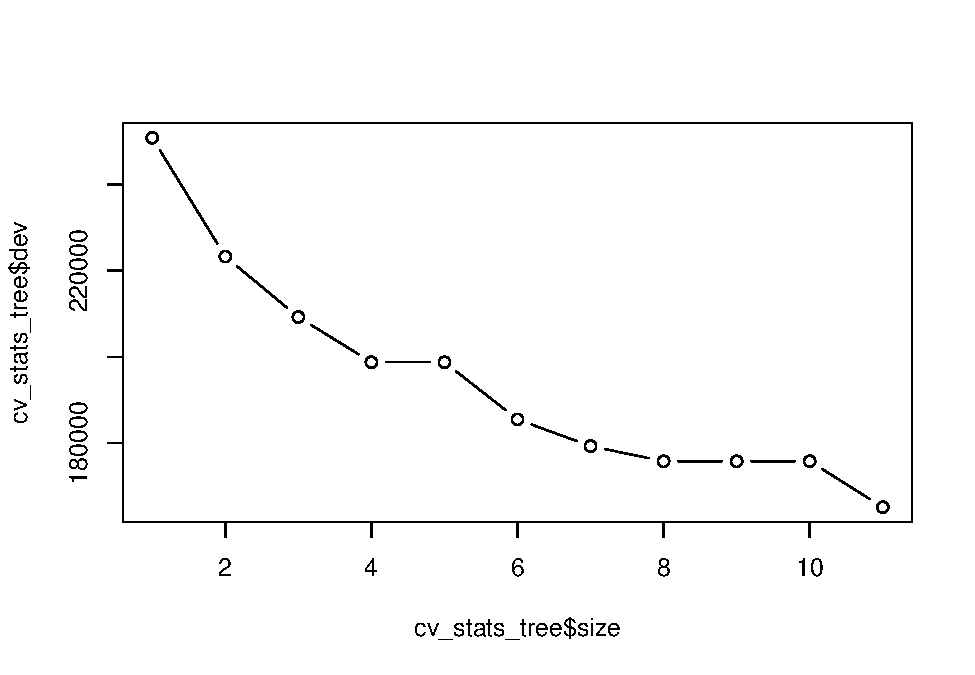
\includegraphics{Regression_files/figure-latex/unnamed-chunk-9-1.pdf}
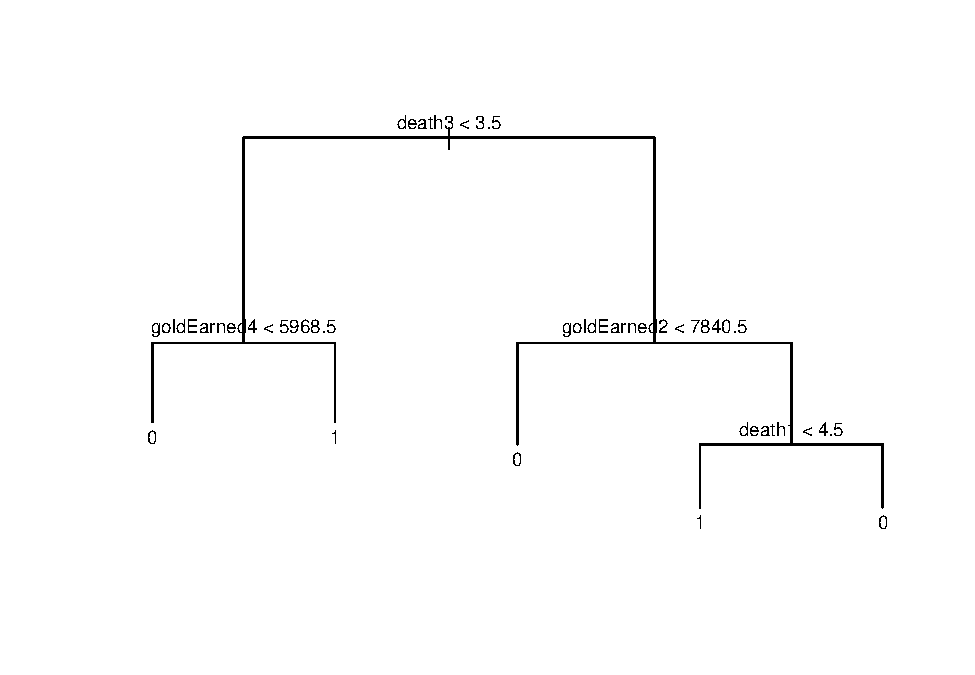
\includegraphics{Regression_files/figure-latex/unnamed-chunk-9-2.pdf}
\includegraphics{Regression_files/figure-latex/unnamed-chunk-9-3.pdf}
\includegraphics{Regression_files/figure-latex/unnamed-chunk-9-4.pdf}

As you can see above these plots are even more extreme in every graph in
the wrong ways. Residuals vs fitted is less of a straight line and
curves dramatically at the end. Normal Q-Q is very much curved at the
edges telling us our dataset is skewed. The scale location is about the
same of a condensed black blob as above. Finally in Residuals vs
Leverage we have even more extreme outliers at both ends, but still no
influential values (barely). Overall with these results this model is
worse than the original above.

\begin{Shaded}
\begin{Highlighting}[]
\NormalTok{lm3 }\OtherTok{\textless{}{-}} \FunctionTok{lm}\NormalTok{(NO2}\SpecialCharTok{\textasciitilde{}}\NormalTok{Year}\SpecialCharTok{+}\NormalTok{PM2}\FloatTok{.5}\SpecialCharTok{+}\NormalTok{PM10, }\AttributeTok{data=}\NormalTok{train)}
\FunctionTok{summary}\NormalTok{(lm3)}
\end{Highlighting}
\end{Shaded}

\begin{verbatim}
## 
## Call:
## lm(formula = NO2 ~ Year + PM2.5 + PM10, data = train)
## 
## Residuals:
##     Min      1Q  Median      3Q     Max 
## -46.932  -5.487  -0.533   2.895 189.527 
## 
## Coefficients:
##               Estimate Std. Error t value Pr(>|t|)    
## (Intercept) 745.837318  44.666035   16.70   <2e-16 ***
## Year         -0.361836   0.022163  -16.33   <2e-16 ***
## PM2.5         0.082272   0.005198   15.83   <2e-16 ***
## PM10          0.071885   0.002708   26.54   <2e-16 ***
## ---
## Signif. codes:  0 '***' 0.001 '**' 0.01 '*' 0.05 '.' 0.1 ' ' 1
## 
## Residual standard error: 9.765 on 25748 degrees of freedom
## Multiple R-squared:  0.05662,    Adjusted R-squared:  0.05651 
## F-statistic: 515.1 on 3 and 25748 DF,  p-value: < 2.2e-16
\end{verbatim}

The summary above can be used to compare this model with the previous
models above. The residual standard error is 9.737 instead of 9.974 and
9.82 on about the same degrees of freedom, this states that roughly the
model's predictions are still about 10 units off being slightly less
than the previous models. The multiple r-squared error is 0.06038, which
is much better than 0.02057 from the first model, and slightly better
than 0.05059 from the second model, this should be as close to 1 as
possible so it is not an improvement compared to the models above. Still
being well under .4 and therefore is still a poor model at explaining
variance in the data. The p-value is for all models is the same that is
significant.

\begin{Shaded}
\begin{Highlighting}[]
\FunctionTok{plot}\NormalTok{(lm3)}
\end{Highlighting}
\end{Shaded}

\includegraphics{Regression_files/figure-latex/unnamed-chunk-11-1.pdf}
\includegraphics{Regression_files/figure-latex/unnamed-chunk-11-2.pdf}
\includegraphics{Regression_files/figure-latex/unnamed-chunk-11-3.pdf}
\includegraphics{Regression_files/figure-latex/unnamed-chunk-11-4.pdf}

As you can see above these plots vary more than the 2nd model. Residuals
vs fitted is less of a straight line and curves more at the end than the
1st model, but is more straight than the 2nd model. Normal Q-Q is very
much curved at the ending edge telling us our dataset is skewed, but not
as bad as the 2nd model. The scale location is about the same of a
condensed black blob as above. Finally in Residuals vs Leverage we have
even more extreme outliers at both ends and has one influential value at
16687. Overall with these results this model is worse than the models
above.

Overall, all of the models do a very poor job at explaining the
variation of the data. Which makes sense as there are many outside
factors not in the dataset that are causing/changing the air
pollution/quality. But the models do manage to have a low p-value and
thus does have a significant meaning and isn't useless. The models
aren't very good in general but could be used for something specific in
predicting the NO2 of areas given PM2.5 or PM10. It is a close call but
we think the 3rd model is the best out of the three as it has a higher
multiple r-squared error and a lower residual standard error.

Here is the testing of the three models:

\begin{Shaded}
\begin{Highlighting}[]
\NormalTok{pred1 }\OtherTok{\textless{}{-}} \FunctionTok{predict}\NormalTok{(lm1, }\AttributeTok{newdata=}\NormalTok{test)}
\NormalTok{pred2 }\OtherTok{\textless{}{-}} \FunctionTok{predict}\NormalTok{(lm2, }\AttributeTok{newdata=}\NormalTok{test)}
\NormalTok{pred3 }\OtherTok{\textless{}{-}} \FunctionTok{predict}\NormalTok{(lm3, }\AttributeTok{newdata=}\NormalTok{test)}
\end{Highlighting}
\end{Shaded}

Here are the test results of the three models: Linear model 1:

\begin{Shaded}
\begin{Highlighting}[]
\NormalTok{correlation1 }\OtherTok{\textless{}{-}} \FunctionTok{cor}\NormalTok{(pred1, test}\SpecialCharTok{$}\NormalTok{NO2)}
\FunctionTok{print}\NormalTok{(}\FunctionTok{paste}\NormalTok{(}\StringTok{"correlation: "}\NormalTok{, correlation1))}
\end{Highlighting}
\end{Shaded}

\begin{verbatim}
## [1] "correlation:  0.135894551778995"
\end{verbatim}

\begin{Shaded}
\begin{Highlighting}[]
\NormalTok{mse }\OtherTok{\textless{}{-}} \FunctionTok{mean}\NormalTok{((pred1 }\SpecialCharTok{{-}}\NormalTok{ test}\SpecialCharTok{$}\NormalTok{NO2)}\SpecialCharTok{\^{}}\DecValTok{2}\NormalTok{)}
\FunctionTok{print}\NormalTok{(}\FunctionTok{paste}\NormalTok{(}\StringTok{"mse: "}\NormalTok{, mse))}
\end{Highlighting}
\end{Shaded}

\begin{verbatim}
## [1] "mse:  101.468859428314"
\end{verbatim}

\begin{Shaded}
\begin{Highlighting}[]
\NormalTok{rmse }\OtherTok{\textless{}{-}} \FunctionTok{sqrt}\NormalTok{(mse)}
\FunctionTok{print}\NormalTok{(}\FunctionTok{paste}\NormalTok{(}\StringTok{"rmse: "}\NormalTok{, rmse))}
\end{Highlighting}
\end{Shaded}

\begin{verbatim}
## [1] "rmse:  10.0731752406237"
\end{verbatim}

Linear model 2:

\begin{Shaded}
\begin{Highlighting}[]
\NormalTok{correlation2 }\OtherTok{\textless{}{-}} \FunctionTok{cor}\NormalTok{(pred2, test}\SpecialCharTok{$}\NormalTok{NO2)}
\FunctionTok{print}\NormalTok{(}\FunctionTok{paste}\NormalTok{(}\StringTok{"correlation: "}\NormalTok{, correlation2))}
\end{Highlighting}
\end{Shaded}

\begin{verbatim}
## [1] "correlation:  0.257559227091291"
\end{verbatim}

\begin{Shaded}
\begin{Highlighting}[]
\NormalTok{mse }\OtherTok{\textless{}{-}} \FunctionTok{mean}\NormalTok{((pred2 }\SpecialCharTok{{-}}\NormalTok{ test}\SpecialCharTok{$}\NormalTok{NO2)}\SpecialCharTok{\^{}}\DecValTok{2}\NormalTok{)}
\FunctionTok{print}\NormalTok{(}\FunctionTok{paste}\NormalTok{(}\StringTok{"mse: "}\NormalTok{, mse))}
\end{Highlighting}
\end{Shaded}

\begin{verbatim}
## [1] "mse:  96.6454082527603"
\end{verbatim}

\begin{Shaded}
\begin{Highlighting}[]
\NormalTok{rmse }\OtherTok{\textless{}{-}} \FunctionTok{sqrt}\NormalTok{(mse)}
\FunctionTok{print}\NormalTok{(}\FunctionTok{paste}\NormalTok{(}\StringTok{"rmse: "}\NormalTok{, rmse))}
\end{Highlighting}
\end{Shaded}

\begin{verbatim}
## [1] "rmse:  9.83083965146214"
\end{verbatim}

Linear model 3:

\begin{Shaded}
\begin{Highlighting}[]
\NormalTok{correlation3 }\OtherTok{\textless{}{-}} \FunctionTok{cor}\NormalTok{(pred3, test}\SpecialCharTok{$}\NormalTok{NO2)}
\FunctionTok{print}\NormalTok{(}\FunctionTok{paste}\NormalTok{(}\StringTok{"correlation: "}\NormalTok{, correlation1))}
\end{Highlighting}
\end{Shaded}

\begin{verbatim}
## [1] "correlation:  0.135894551778995"
\end{verbatim}

\begin{Shaded}
\begin{Highlighting}[]
\NormalTok{mse }\OtherTok{\textless{}{-}} \FunctionTok{mean}\NormalTok{((pred3 }\SpecialCharTok{{-}}\NormalTok{ test}\SpecialCharTok{$}\NormalTok{NO2)}\SpecialCharTok{\^{}}\DecValTok{2}\NormalTok{)}
\FunctionTok{print}\NormalTok{(}\FunctionTok{paste}\NormalTok{(}\StringTok{"mse: "}\NormalTok{, mse))}
\end{Highlighting}
\end{Shaded}

\begin{verbatim}
## [1] "mse:  95.6764517052423"
\end{verbatim}

\begin{Shaded}
\begin{Highlighting}[]
\NormalTok{rmse }\OtherTok{\textless{}{-}} \FunctionTok{sqrt}\NormalTok{(mse)}
\FunctionTok{print}\NormalTok{(}\FunctionTok{paste}\NormalTok{(}\StringTok{"rmse: "}\NormalTok{, rmse))}
\end{Highlighting}
\end{Shaded}

\begin{verbatim}
## [1] "rmse:  9.78143403112459"
\end{verbatim}

As expected the correlation for all models is quite low, the highest is
model 2, but is still very unacceptable. The RMSE tells us that our
model is off around 10 units as expected from above. We believe these
results happened because there was a lot of missing data in the dataset
that we had to fill in with medians, as well as the unpredictable
differences between these data values. They are primarily caused by
outside forces, not necessarily by each other therefore there is likely
little accurate correlation between them and using them to predict
another is ignoring outside factors. There was also a very high amount
of variance in the data that very much affected the ability for the
linear model to fit the dataset well.

\end{document}
